\section{Оборудование}
\begin{figure}[ht!]
    \center{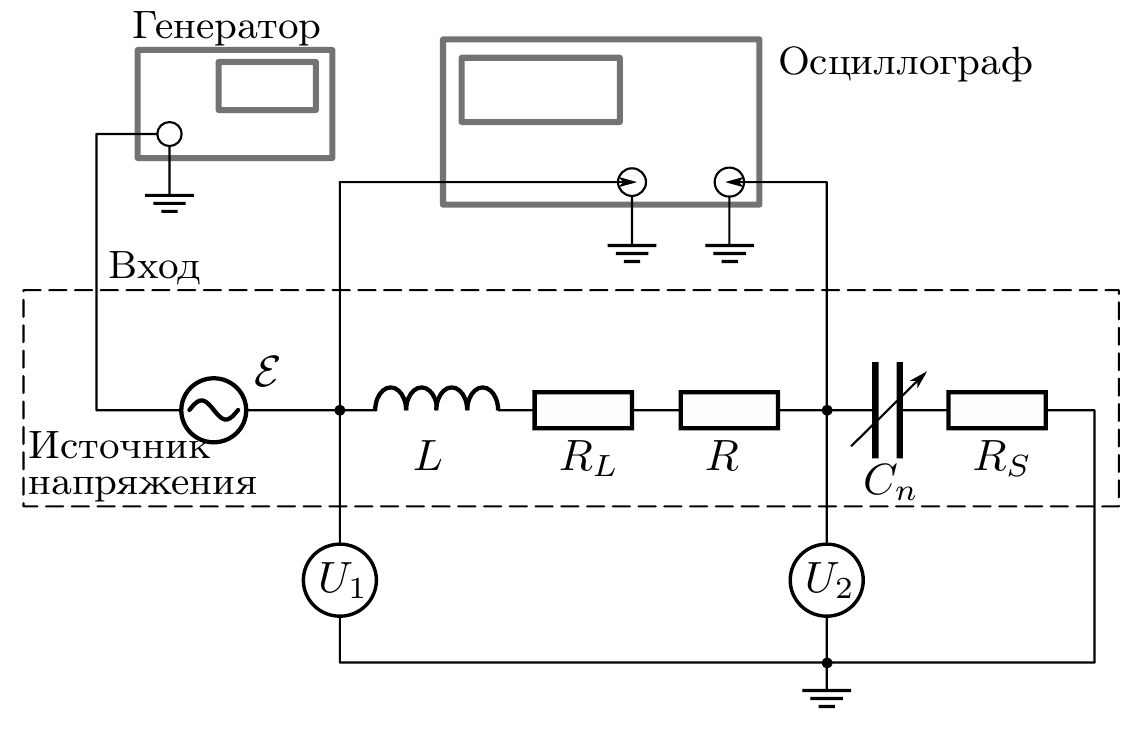
\includegraphics[width=0.8\linewidth]{../img/fig1.png}}
\end{figure}

Схема установки приведена на рисунке.

Синусоидальный сигнал от генератора поступает на вход управляемого напряжением источника напряжения, собранного на операционном усилителе, питание которого осуществляется встроенным блоком-выпрямителем от сети.
Источник напряжения обеспечивает с высокой точностью постоянство амплитуды сигнала $ \varepsilon = \varepsilon_{0} \cos \left( \omega t + \varphi_{0}\right)$ на меняющейся по величине нагрузке (последовательном колебательном контуре).

Источник напряжения, колебательный контур и блок питания заключены в отдельный корпус, отмеченный на рисунке штриховой линией. На корпусе имеются коаксиальные разъёмы и <<Вход>>, <<$U_{1}$>> и <<$U_{2}$>>, а также переключатель магазина
ёмкостей $C_{n}$ с указателем номера. Величины ёмкостей указаны на установке. Напряжение $ \varepsilon $ на контуре через разъём <<$U_{1}$>> попадает одновременно на канал 1 осциллографа и вход 1-го цифрового вольтметра. Напряжение на
конденсаторе $U_{C}$ подаётся через разъём <<$U_{2}$>> одновременно на канал 2 осциллографа и вход 2-го цифрового вольтметра.

\textbf{Особенности реальных элементов цепи.} Колебательный контур  собран из стандартных элементов, используемых в современных радиоэлектронных цепях. Известно, что в реальных конденсаторах и особенно в катушках индуктивности происходят
необратимые потери энергии. К ним относятся: утечки и диэлектрические потери в конденсаторах, вихревые токи и потери на перемагничивание в сердечниках катушек индуктивности, омические потери в проводниках, растущие с частотой за счёт
скин-эффекта и т.д. Рост потерь приводит к увеличению действительных частей комплексных сопротивлений элементов контура и, значит, к изменению его резонансных свойств, в частности, к уменьшению добротности.

Потери в элементах контура зависят как от частоты, так и от амплитуды тока (напряжения),  температуры и ряда других факторов. В общем случае зависят индуктивность $L$, ёмкость $C$ и суммарное сопротивление $R_{ \Sigma }$.

В контуре катушка индуктивности $L$ обладает малым сопротивлением по постоянному току и высокой собственной резонансной частотой $ \nu_{L0}>1{,}3\,\text{МГц}$.
Помимо индуктивности каждая катушка характеризуется собственной ёмкостью $C_{L}$ и активным сопротивлением $R_{L}$. Принимается, что эти величины сосредоточены в отдельных элементах схемы, образующих с индуктивностью
замкнутую колебательную цепь с собственной резонансной частотой $ \nu_{L0}=1/2 \pi \sqrt{LC_{l}}$.
Вследствие влияния ёмкости $C_{L}$ при измерении на частоте $ \nu $ определяется не истинная индуктивность $L$, а эффективное значение индуктивности $L_{\text{эфф}}=L/\left(1- \nu^{2}/\nu^{2}_{0}\right)$,  которое может заметно
отличаться от истинной величины $L$.

В этой работе $ \nu \ll \nu_{0}$, поэтому индуктивность представлена последовательным соединением $L$ и $R_{L}$.

\begin{figure}[ht!]
    \center{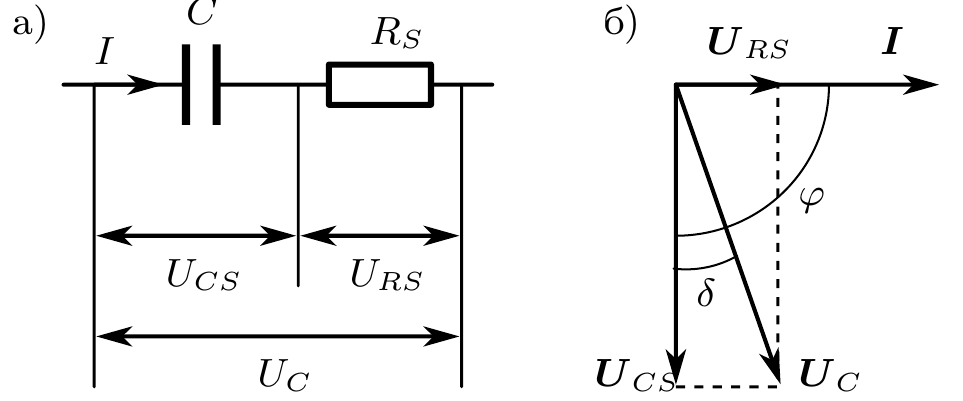
\includegraphics[width=0.8\linewidth]{../img/fig2.png}}
\end{figure}

Конденсаторы $C_{n}$ имеют пренебрежимо малые собственные индуктивности и относительно малые активные потери. Для оценки вклада активных потерь можно представить конденсатор как последовательное соединение конденсатора
$C$ и сопротивления $R_{S}$. Из рисунка видно, что активные потери в конденсаторе, пропорциональные косинусу угла $ \varphi $, убывают с ростом $ \varphi $. Потери в конденсаторе принято характеризовать величиной
$\tg \delta $, $ \delta = \frac{ \pi }{2} - \varphi $.
\[
    R_{S} = \frac{U_{RS}}{I} = \frac{U_{RS}}{ \omega C U_{CS}} = \frac{\tg \delta }{ \omega C}
\]

В работе $\tg \delta < 10^{-3}$.

\textbf{Свойства колебательного контура.} В колебательный контур добавлен постоянный резистор $R$, снижающий его добротность.
\[
    R_{ \Sigma } = R + R_{L} + R_{S}
\]

\[
Q = \frac{ \rho }{R_{ \Sigma }} = \frac{ \omega_{0}L}{R_{ \Sigma }} = \frac{1}{ \omega_{0} C R_{ \Sigma }} \gg 1
\]

Для импедансов ёмкости $Z_{C}$ и индуктивности $Z_{L}$ и последовательного контура $Z=Z_{L}+R+Z_{C}$ верны выражения
\[
    Z_{C} = R_{S} - \frac{i}{ \omega C}
\]
\[
    Z_{L} = R_{L} + i \omega L
\]
\[
    Z = R_{ \Sigma } + i\left( \omega L - \frac{1}{ \omega C}\right)
\]

\[
    I = \frac{U_{R}}{R} = \frac{ \varepsilon_{0}}{R_{ \Sigma }}\frac{1}{1+iQ\left( \omega / \omega_{0} - \omega_{0} / \omega \right)}
\]
\[
    U_{C} = -iQ \varepsilon_{0}\frac{ \omega_{0}}{ \omega }\frac{1+i\tg \delta }{1 + iQ\left( \omega / \omega_{0} - \omega_{0} / \omega \right)}
\]
\[
    U_{L} = iQ \varepsilon_{0}\frac{ \omega }{ \omega_{0}}\frac{1-iR_{L}/ \rho }{1 + iQ\left( \omega  / \omega_{0} - \omega_{0} / \omega \right)}
\]

При $Q\gg 1$ и $\tg \delta < 10^{-3}$ мнимыми добавками к потере можно пренебречь. Но нужно оценить их вклад вблизи резонанса, равный примерно $R_{L} + \rho \tg \delta $.

Наибольший практический интерес представляет случай, когда
\[
    \left| \omega - \omega_{0}\right| = \left| \Delta \omega \right| \ll \omega_{0}
\]
При этом в первом порядке малости по $ \Delta \omega / \omega_{0}$
\[
    \frac{ \omega }{ \omega_{0}} - \frac{ \omega_{0}}{ \omega } = \frac{2 \Delta \omega }{ \omega_{0}}
\]

Это позволяет представить вещественные части комплексных амплитуд в виде
\[
    I = \frac{ \varepsilon_{0}}{R_{ \Sigma }}\frac{\cos\left( \omega t - \psi_{I}\right)}{\sqrt{1 + \left( \tau \Delta \omega \right)^{2}}}
\]
\[
    \psi_{I} = \arctg \left( \tau \Delta \omega \right)
\]
\[
    U_{C} = Q \varepsilon_{0} \frac{ \omega_{0}}{ \omega }\frac{\cos \left( \omega t - \psi_{C}\right)}{\sqrt{1 + \left( \tau \Delta \omega \right)^{2}}}
\]
\[
    \psi_{C} = \psi_{I} + \frac{ \pi }{2} - \delta 
\]
\[
    U_{L} = Q \varepsilon_{0} \frac{ \omega }{ \omega_{0}}\frac{\cos\left( \omega  t - \psi_{L}\right)}{\sqrt{1 + \left( \tau \Delta \omega \right)^{2}}}
\]
\[
    \psi_{L} = \psi_{I} - \frac{ \pi }{2} + \frac{R_{L}}{ \rho }
\]
\[
    \tau = \frac{2L}{R}
\]
$ \tau $~--- время затухания.

В резонансе модули комплексных амплитуд принимают вид
\[
    I( \omega_{0}) = \frac{U_{R}}{R}
\]
\[
    U_{C}( \omega_{0}) = Q \varepsilon_{0}
\]
\[
    U_{L}( \omega_{0}) = Q \varepsilon_{0}
\]
В резонансе контур становится чисто активным и $I_{max} = \varepsilon_{0}/R_{ \Sigma }$. Напряжения $U_{L}$ и $U_{C}$ на частоте $ \omega_{0}$ находятся почти в противофазе и в $Q$ раз по амплитуде
превышают $ \varepsilon $ внешней ЭДС (с поправкой порядка $Q^{-2}$).

При таком отклонении, что
\[
    \tau \Delta \omega = \pm 1
\]
амплитуда тока $I$ уменьшается в $\sqrt{2}$ раз относительно резонансной величины, а фаза $ \psi_{I}$ меняется на угол $\pm \pi /4$. В этой же точке происходят аналогичные изменения амплитуд $U_{C}$, $U_{L}$ и фаз
$ \psi_{C}$ и $ \psi_{L}$ напряжений на  ёмкости и индуктивности: амплитуды уменьшаются в $\sqrt{2}$ раз, а фазы меняются на угол $\pm \pi /4$ по отношению к своим резонансным значениям.

Величина $ \delta \omega  = 2 | \Delta  \omega | = 2 / \tau $ является шириной резонансной кривой $U_{C}( \omega )$ на уровне $U_{C}( \omega_{0})/\sqrt{2}$, по которой можно определить время затухания $ \tau  = 2 / \delta \omega $
и найти добротность контура $Q = \omega_{0} / \delta \omega $.

Эти же параметры можно определить по фазово-частотной характеристике: расстояние по оси $ \omega $ между точками, в которых фаза $ \varphi_{C}$ меняется от $- \pi /4$ до $3 \pi / 4$ равно $2 \tau $,
а тангенс угла наклона функции $ \varphi_{C}( \omega)$ в точке резонанса определяет время затухания.

В работе резонансные явления в последовательном колебательном контуре исследуются по напряжению на контуре $ \varepsilon $ и напряжению на ёмкости $U_{C}$, а также по фазовым сдвигам между ними.
